\section{Discussion}

\subsection{Ambiguity in Standards}
While determining how to interpret the NIST standards, we encountered ambiguities in their current wording.
The first issue concerns core feature 3. 
Particularly, ``all non-allocated data blocks identified in a residual metadata entry''\cite{meta:dfr:standards} is not well-defined when considering a FAT filesystem. 
In FAT, the only relevant metadata left over after file deletion is the address of the first cluster of file data, and the file's length. 
If the deleted file is fragmented at any point, no evidence remains in the metadata. 
Therefore, interpreting the wording very closely, a tool is only required to recover the first cluster of a file's data. 
As this would not be particularly useful, it is unlikely that this was the intended meaning. 
For these tests we interpret core feature 3 as requiring the first contiguous segment of unallocated sectors starting from the first sector originally allocated to the deleted file. 
In other words, if the file is fragmented, the tool must recover at least the first fragment. 
If a file is partially overwritten, the tool must recover at least the sectors before the overwritten part. 
However, it should be emphasized this is an assumption and the intent of the standard in this case should be clarified.

Furthermore, there are situations in which core features 3 and 4 are entirely incompatible. 
Core feature 3 specifies ``all non-allocated data blocks identified in a residual metadata entry,''\cite{meta:dfr:standards} but that can sometimes still include data from other files. 
One such situation is when a deleted file is overwritten, and then the overwriting file is also deleted, such as in case 5i. ~\ref{fig:case_5i}

\begin{figure}[h]
    \centering
    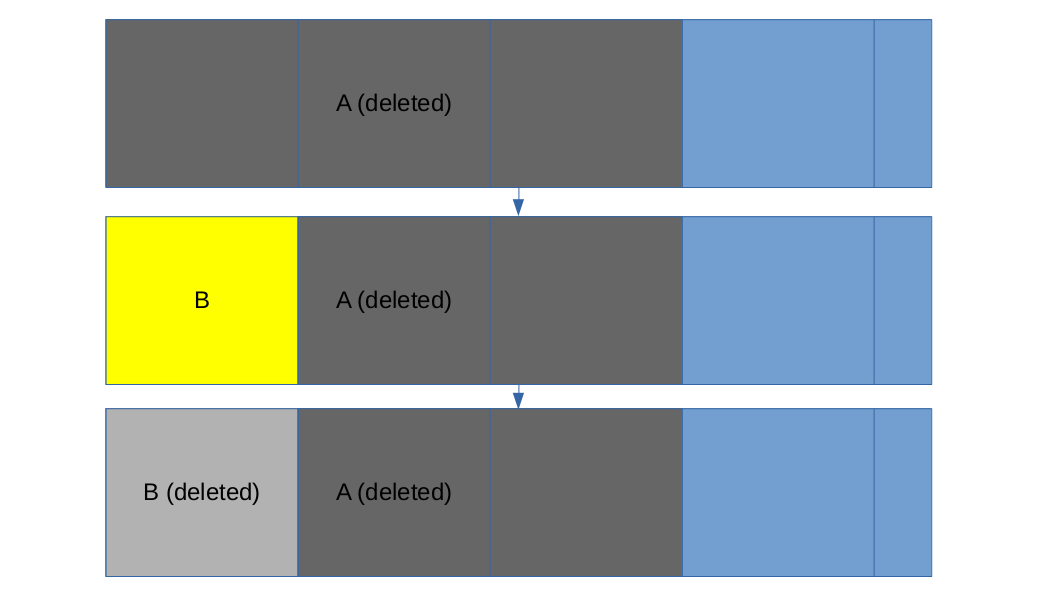
\includegraphics[width=\linewidth]{fig/case5i.png}
    \caption{Test Case 5i}
    \label{fig:case_5i}
\end{figure}

Assuming the filesystem is NTFS (to avoid the afforementioned ambiguity with core feature 3 and FAT), the residual metadata entry for File A (in this case its Master File Table entry) should list every sector File A once occupied, and all of those sectors are unallocated. 
To fulfill core feature 3, the tool must recover all of those sectors. 
However, some of those sectors have been overwritten by File B. Core feature 4 requires that a tool only recover ``data blocks from the Deleted Block Pool,''\cite{meta:dfr:standards} and limits the definition of Deleted Block Pool to blocks which ``have not been reallocated or reused.``\cite{meta:dfr:standards}
Core feature 3 would require tools to recover the sectors reused by File B, while core feature 4 would forbid this. 
It could be argued that the tool should use File B's metadata to recognize that File B overwrote File A, but this is not always realistic. 
While the filesystem stores information such as creation and modification times, this is not ''essential metadata,`` meaning it is not involved in the operation of the filesystem, so operating systems may implement it differently, or not at all. % TODO cite Carrier on definition of non-essential metadata
Since the time information cannot be counted on to be reliable, there is no way to know for sure which file overwrote which. It is also possible for file B's metadata entry to be overwritten at some point before File A's, in which event there is no way for the tool to know File B even existed.
%TODO wrap this up better, mention standards document's ''recovered object`` definition and how it does acknowledge possible data corruption

The NIST standards should be revised to account for situations where core features are in contradiction.
\comment{Should we suggest specific revisions?}
